% Gallery figure source
% Summary: Reassortment assigns entire genome segments to parental lineages. It is especially important for segmented viruses such as influenza A.
\documentclass[tikz,border=6pt]{standalone}
% Shared color palette
\usepackage[T1]{fontenc}
\usepackage[utf8]{inputenc}
\usepackage{lmodern}
\usepackage{microtype}
\usepackage{amsmath,amssymb,mathtools}
\usepackage{xcolor}
\usepackage{tikz}
\usetikzlibrary{arrows.meta,positioning,calc,fit,backgrounds,decorations.pathreplacing,shapes.geometric,shadows.blur}

\definecolor{mainblue}{RGB}{42,85,132}
\definecolor{deepgreen}{RGB}{30,105,70}
\definecolor{burntorange}{RGB}{190,90,25}
\definecolor{softgray}{RGB}{245,246,248}
\definecolor{darkgray}{RGB}{70,70,70}
\definecolor{violet}{RGB}{110,70,150}

\newcommand{\given}{\,|\,}
\newcommand{\Ne}{N_{e}}
\newcommand{\ARG}{\mathrm{ARG}}
\newcommand{\MRCA}{\mathrm{MRCA}}
\newcommand{\GMRCA}{\mathrm{GMRCA}}

% Shared TikZ styles
\tikzset{
  tip/.style={circle,fill=black,inner sep=1.6pt},
  nodept/.style={circle,fill=black,inner sep=1.4pt},
  sampled/.style={rectangle,fill=black,inner sep=2.2pt},
  branch/.style={line width=0.8pt},
  retic/.style={circle,draw=burntorange,fill=burntorange!25,line width=0.8pt,inner sep=2.0pt},
  event/.style={circle,draw=mainblue,fill=mainblue!15,line width=0.8pt,inner sep=1.8pt},
  arr/.style={-{Latex[length=2.0mm]},line width=0.8pt},
  faint/.style={line width=0.7pt,draw=gray!55},
  parentedge/.style={-{Latex[length=2.0mm]},line width=0.9pt,draw=burntorange},
  treeedge/.style={-{Latex[length=2.0mm]},line width=0.9pt,draw=black},
  segment/.style={line width=4pt,line cap=round},
  dashedretic/.style={-{Latex[length=2.0mm]},line width=0.9pt,draw=burntorange,dashed}
}


\begin{document}
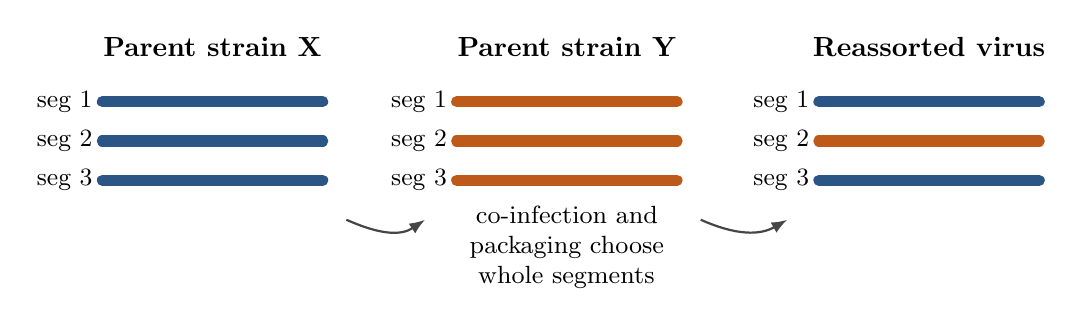
\begin{tikzpicture}[scale=1.0]
  \node[font=\bfseries] at (1.7,3.2) {Parent strain X};
  \foreach \y/\lab in {2.5/seg 1,2.0/seg 2,1.5/seg 3}{
    \draw[segment,mainblue] (0.3,\y)--(3.1,\y);
    \node[left,font=\small] at (0.3,\y) {\lab};
  }
  \node[font=\bfseries] at (6.2,3.2) {Parent strain Y};
  \foreach \y/\lab in {2.5/seg 1,2.0/seg 2,1.5/seg 3}{
    \draw[segment,burntorange] (4.8,\y)--(7.6,\y);
    \node[left,font=\small] at (4.8,\y) {\lab};
  }
  \node[font=\bfseries] at (10.8,3.2) {Reassorted virus};
  \draw[segment,mainblue] (9.4,2.5)--(12.2,2.5); \node[left,font=\small] at (9.4,2.5) {seg 1};
  \draw[segment,burntorange] (9.4,2.0)--(12.2,2.0); \node[left,font=\small] at (9.4,2.0) {seg 2};
  \draw[segment,mainblue] (9.4,1.5)--(12.2,1.5); \node[left,font=\small] at (9.4,1.5) {seg 3};
  \draw[arr,draw=darkgray] (3.4,1.0) .. controls (3.85,0.8) and (4.1,0.8) .. (4.4,1.0);
  \draw[arr,draw=darkgray] (7.9,1.0) .. controls (8.35,0.8) and (8.65,0.8) .. (9.0,1.0);
  \node[align=center,font=\small,text width=3.4cm] at (6.2,0.65) {co-infection and packaging choose whole segments};
\end{tikzpicture}
\end{document}
